%capitulo03
\label{cap:researchproblems}
\noindent
This section presents the research problems found in the state of the art of the runtime systems that shall be explored during the doctoral studies. Table~\ref{tab:problems} summarises the properties involved in these research directions. First, it is presented the research problems in the context of properties regarding efficiency, after, regarding of the fairness execution.

\begin{table}[hbtp]
	\centering
	\caption{Research problems.}
	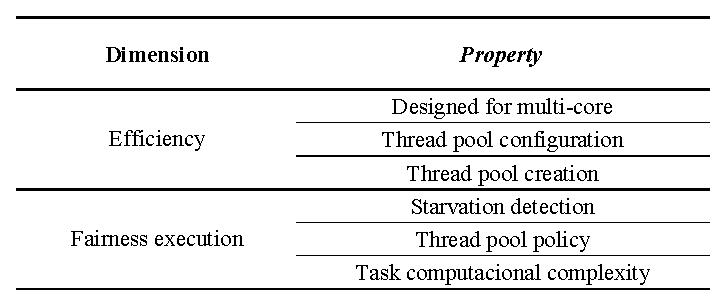
\includegraphics[scale=0.9]{./figs/issues.eps}
	%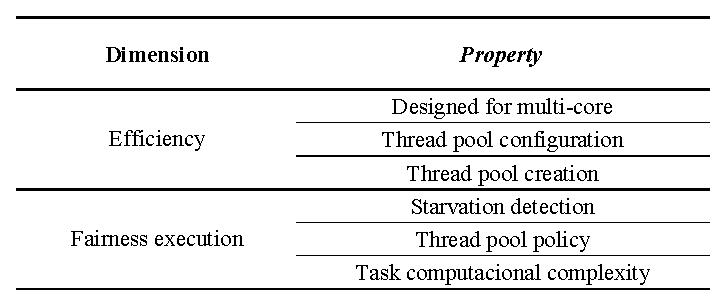
\includegraphics[width=\linewidth]{./figs/issues.eps}
\label{tab:problems}%
\end{table}%

%==============================================================================
\section{{Directions on Efficiency}}
\label{sec:directions_efficiency}
%==============================================================================
Software engineers seek to develop algorithms that can take full advantage of multi-core design so that achieve a high level of parallelism and an overall high performance. The way the algorithms are written impact in the success of multi-core technology strongly~\cite{sethi2015}. Design multi-core is a property, which should be present in runtime systems bearing in mind that the technological advances already offers resources to extends the parallel program. For hardware, modern technologies as Graphics processing units (GPUs) can be cited, which demand tens of thousands of concurrent threads to fully utilize the massive amount of processing resources~\cite{yoon2016}. GPUs hold great massively parallel computing capabilities, with potential for the acceleration of computationally intensive algorithms~\cite{tang2017}. 

Some works are shown promising proposals of thread pool configuration models, like the article of Nazeer et al.~\cite{nazeer2016}, which achieves good results in simulations, with the named Hybrid scheme to dynamically, which optimize a thread pool, based on predicting incoming request frequencies. Gleyzer et al.~\cite{gleyzer2017} propose a method allows dynamic thread pool sizing suitable for use in multi-threaded processing environment such as a distributed data grid. The method utilizes measurements of thread pool throughput and measurements of worker thread utilization in combination with analysis of prior thread pool resizing actions to determine whether to add or remove worker threads from a thread pool in a current resizing action. The method claims a rapid and responsive adjustment of thread pool size in response to changes in workload and processor availability. These works motivate us to deepen our research, so that the thread pool configuration of the runtime systems of the integration platforms occurs elastically, following the demand of processing the tasks and thus, using the computational resources more efficiently.

The research of Lee et al.~\cite{lee2011} shows better response time and CPU usage, by means prediction of the number of threads and thread pool management. Trendy exponential moving average (TEMA) scheme, proposed by Lee et al., adjusts the idle time out period and thread pool size to adapt the system to the changing environment. The article of Oh and Kim~\cite{oh2013} presents a history-based dynamic method (HisDyn), which minimizes throughput degradation, due to creation of threads, by means of estimation and maintenance of the number of threads needed for requests. HisDyn predicts the range of needed threads, through of the mean task arrival times and mean task processing times.

Bahadur et al.~\cite{bahadur2014} propose a thread pool system able of dynamic optimization thread pool size, according request frequencies, named Frequency Based Optimization Strategy (FBOS). After, Ashraf et al.~\cite{ashraf2016} present an extension of work of FBOS, namely Non-blocking Frequency Based Optimization Strategy with Automated Timers (NBFBOS with Automated Timers), which dynamically optimises thread pool, using of non-blocking synchronization primitives offering advantages of substantial scalability and liveliness. For all this, it is possible to find out to get optimised strategies to create threads at runtime to runtime systems of integration platforms.

%==============================================================================
\section{{Directions on Fairness Execution}}
\label{sec:directions_fairness}
%==============================================================================
Shah et al.~\cite{shah2017} argue that when starvation occurs it decreases response time and increases wait time to execution of requests and propose to explore the implementation of multiple thread pools based on a distribution of service times to avoid starvation and achieve concurrency of processing. Their analysis showed that proposed scheme is increases the response time and reduces the wait time. This research endorses the need and possibility of the runtime systems detecting starvation detection, therefore, the detection starvation is a potential field of study.

Tsai et al.~\cite{tsai2013} propose to optimize task scheduling and resource allocation using an improved differential evolution algorithm (IDEA), based on the proposed cost and time models on cloud computing environment. Elmougy et al.~\cite{elmougy2017} propose a novel hybrid task scheduling algorithm named (SRDQ) combining Shortest-Job-First (SJF) and Round Robin (RR) schedulers considering a dynamic variable task quantum. Singh et al.~\cite{singh2017} present a review of using meta-heuristics techniques for scheduling tasks in cloud computing, based on swarm intelligence and bio-inspired techniques and claim that it is possible to decide suitable approach for better schemes for scheduling according to the application. These works encourages us to pursue smarter policies to schedule tasks for the thread pools in the runtime systems of integration platforms.

Cordes et al.~\cite{cordes2011} claim that it is essential to balance the execution time of all tasks in a work flow of processing running in parallel in order to achieve the best possible utilization of computing resources. The proposed method by authors employs a cost model that allows incorporating differing execution times for loop iterations of the program due to the underlying heterogeneous platform. The consideration of execution time heterogeneity enables the in parallel approach to using each processing unit according to its performance characteristics in a system as well as the utilization of as many processing units as possible simultaneously.

Sudarsanam et al.~\cite{sudarsanam2004} address the compatibility between resource and task by estimating the amount of resources that are needed for a reconfigurable architecture to suit task granularity. These studies point out that considering the computational complexity to be executed can lead to a better allocation of computational resources.